% !TeX spellcheck = en_US
% Here and after: russian-aot is available here: https://extensions.openoffice.org/de/download/18162

\documentclass[14pt]{extreport}

\usepackage[legalpaper, left=3cm, right=1.5cm, top=2cm, bottom=1.25cm, includefoot]{geometry}

\usepackage[utf8]{inputenc}
\usepackage[T1, T2A]{fontenc}
\usepackage[main=russian, english, german, latin]{babel}
\usepackage{tempora, newtxmath}

\usepackage{tabularx, xltabular, multirow, makecell}
\usepackage[compact]{titlesec}
\usepackage[inline]{enumitem}
\usepackage{tocloft}

\usepackage{ulem}
\usepackage{contour}
\usepackage{setspace}
\usepackage{csquotes}

\usepackage{totcount}
\usepackage{listings}

\usepackage{array}
\usepackage{xinttools}

\usepackage{caption}
\usepackage{tikz}
\usetikzlibrary{positioning, fit, backgrounds, calc}
\graphicspath{{./images/}}

% \usepackage{showkeys}
\usepackage[hyphens]{url}
\usepackage[unicode, colorlinks=true, linkcolor=, urlcolor=blue, citecolor=]{hyperref}
\hypersetup {
	pdfauthor={Сергеев А. Д.},
	pdftitle={Разработка программной системы наблюдения за распространением потенциально опасных для человека видов растений},
	pdfsubject={Удобство и скорость отправки и получения данных},
	pdfkeywords={Опасные для человека растения, Мобильное приложение, Django, DRF, PostGIS, Flutter, BLoC, TensorFlow, Docker}
}

% !TeX spellcheck = en_US

\makeatletter
\def\trueonehalfspace{1.213}

\newcommand{\titlelongtext}[1]{\begin{spacing}{\trueonehalfspace}#1\end{spacing}}

\newcommand{\@subscript}[1]{
	\fontsize{12}{14.4}\centering{\textit{\textsuperscript{#1}}}
}

\newcommand{\emptydate}{
	\textquote{\uline{\hspace{1cm}}} \uline{\hspace{3cm}} 2022 г.
}

\newcommand{\worktitle}[1]{
	\begin{tabularx}{\textwidth}{ X X }
		Студент \hspace{1cm} Сергеев А. Д. & \raggedleft{Группа 8304}
	\end{tabularx}
	\begin{tabularx}{\textwidth}{ X }
		\titlelongtext{
			Тема работы: Разработка программной системы наблюдения за распространением потенциально  опасных для человека видов растений
		}
		#1
	\end{tabularx}
}

\newcommand{\subsblock}{
	\begin{tabularx}{\textwidth}[t]{ X X X X }
		Студент & & & Сергеев А. Д. \\ \cline{3-3}
		& & \@subscript{(подпись)} & \\
		Руководитель & \centering{к.т.н., доцент} & & Заславский М. М. \\ \cline{3-3}
		& \@subscript{(Уч. степень, уч. звание)} & \@subscript{(подпись)} & \\
		Консультант & & & Черепанов И. В. \\ \cline{3-3}
		& & \@subscript{(подпись)} & \\
		Консультант & \centering{к.т.н., доцент} & & Заславский М. М. \\ \cline{3-3}
		& \@subscript{(Уч. степень, уч. звание)} & \@subscript{(подпись)} & \\
	\end{tabularx}
}

\newcommand{\confirmation}{
	\setlength{\extrarowheight}{0.25cm}
	\begin{tabularx}{\textwidth}{ X r }
		& Утверждаю \\
		& Зав. кафедрой МО ЭВМ \\
		& \uline{\hspace{3cm}} Кринкин К. В. \\
		& \emptydate
	\end{tabularx}
}



\let\latex@input\input
\newcommand\current@input[1]{\def\currentfile{#1} \par\nobreak\latex@input{#1}%
}
\AtBeginDocument{\let\input\current@input}



\newcommand{\defineterm}[2]{\label{def:#1}\hyperref[lnk:#1]{#2}}
\newcommand{\linkterm}[2]{\label{lnk:#1}\hyperref[def:#1]{\textbf{#2}}}

\newcommand{\tab}{\hspace{0.5cm}}
\newcommand{\nwln}{\vspace{\baselineskip}\tab}

\newcommand{\longcaption}[1]{
	\caption{#1}
	\addtocounter{table}{-1}
	\endfirsthead
	\caption*{Продолжение таблицы \arabic{table}}
	\endhead
}



\titleformat{\section}[hang] {\centering\bfseries}{\thesection\ } {0pt}{\MakeUppercase}
\titleformat{\subsection}[hang] {\bfseries}{\thesubsection\ } {0pt}{}
\renewcommand{\thesection}{\arabic{section}}

\newcommand{\@newcont}[1]{\addcontentsline{toc}{section}{#1}}
\newcommand{\@newcontsect}[1]{\phantomsection\section*{#1}\@newcont{#1}}
\newcommand{\@newcontnosect}[1]{\phantomsection\@newcont{#1}}
\newcommand{\newcont}{\@ifstar{\@newcontnosect}{\@newcontsect}}



\addto\captionsrussian{\renewcommand{\figurename}{Рисунок}}

\tikzset{node distance = 3.5cm and 5.5cm}
\tikzset{block/.style = {draw, minimum height=1.5cm, text width=3cm, align=center}}
\tikzset{block/.style = {draw, minimum height=1.5cm, text width=3cm, align=center}}
\tikzset{link/.style = {minimum height=1cm, text width=2.25cm, midway, align=center}}



\titleformat{\chapter}[display] {\centering\bfseries}{} {0pt}{\MakeUppercase}
\titlespacing*{\chapter}{0pt}{-\baselineskip}{0pt}

\let\@thebibliography\thebibliography
\renewcommand\thebibliography[1]{
	\@thebibliography{#1}
	\setlength{\parskip}{0pt}
	\setlength{\itemsep}{0pt plus 0.3ex}
}

\renewcommand\bibname{Список литературы}
\newcommand{\webbibitem}[4]{\bibitem{#1} \href{#2}{#2} // #3, дата обращения: #4}
\makeatother


\begin{document}
	\setlength\parindent{0pt}
	
	\begin{center}
	\fontsize{13}{15.6}\textbf{
		«Санкт-Петербургский государственный электротехнический университет \\
		«ЛЭТИ» им. В.И.Ульянова (Ленина)» \\
		(СПбГЭТУ «ЛЭТИ»)
	}

	\vspace*{2cm}

	\setlength{\extrarowheight}{0.25cm}
	\begin{tabularx}{\textwidth}{ X X }
		\textbf{Направление} & 09.03.04 \\
		\textbf{Профиль} & Программная инженерия \\
		\textbf{Факультет} & ФКТИ \\
		\textbf{Кафедра} & МО ЭВМ \\
		\textit{К защите допустить} & \\
		Зав. кафедрой & {\raggedleft{Иванов И. И.}}
	\end{tabularx}

	\vspace*{3cm}
	
	\fontsize{18}{21.6}\textbf{
		ВЫПУСКНАЯ КВАЛИФИКАЦИОННАЯ РАБОТА \\
		БАКАЛАВРА
	}

	\vspace*{1cm}
	
	\textbf{
		Тема: наименование темы
	}

	\vspace*{5cm}
	
	\subsblock

	\vspace*{5cm}
	
	Санкт-Петербург \\
	2022
\end{center}

\clearpage

	\begin{center}
	\textbf{
		ЗАДАНИЕ \\
		НА ВЫПУСКНУЮ КВАЛИФИКАЦИОННУЮ РАБОТУ
	}

	\vspace*{2cm}

	\setlength{\extrarowheight}{0.25cm}
	\begin{tabularx}{\textwidth}{ X X }
		& Утверждаю \\
		& Зав. кафедрой МО ЭВМ \\
		& \uline{\hspace{3cm}} Иванов И. И. \\
		& \emptydate
	\end{tabularx}

	\vspace*{3cm}
	
	\begin{tabularx}{\textwidth}{ X X }
		Студент \hspace{1cm} Сергеев А. Д. & \raggedleft{Группа 8304}
	\end{tabularx}

	\begin{tabularx}{\textwidth}{ X }
		Тема работы: Наименование темы \\
		Место выполнения ВКР: место выполнения ВКР \\
		Исходные данные (технические требования): \\
		кратко указываются основные требования к ВКР \\
		Содержание ВКР: \\
		Кратко перечисляются основные разделы ВКР \\
		Перечень отчетных материалов: пояснительная записка, \\ иллюстративный материал, иные отчетные материалы \\
		Дополнительные разделы: указывается наименование \\ дополнительного раздела
	\end{tabularx}

	\vspace*{2cm}
	
	\begin{tabularx}{\textwidth}{ X X }
		Дата выдачи задания & Дата представления ВКР к защите \\
		\emptydate & \emptydate
	\end{tabularx}

	\vspace*{3cm}

	\begin{tabularx}{\textwidth}[t]{ X X X X }
		Студент & & & Сергеев А. Д. \\ \cline{3-3} \\
		Руководитель & & & Иванов И. И. \\ \cline{3-3}
		& \subscript{(Уч. степень, уч. звание)} & & \\
		Консультант & & & Иванов И. И. \\ \cline{3-3}
		& \subscript{(Уч. степень, уч. звание)} & & \\
	\end{tabularx}
\end{center}

\clearpage

	\begin{center}
	\textbf{
		КАЛЕНДАРНЫЙ ПЛАН ВЫПОЛНЕНИЯ \\
		ВЫПУСКНОЙ УВАЛИФИКАЦИОННОЙ РАБОТЫ
	}

	\vspace*{2cm}

	\confirmation

	\vspace*{3cm}
	
	\worktitle

	\vspace*{4cm}
	
	\begin{tabularx}{\textwidth}{ l X l }
		№ п/п & Наименование работ & Срок выполнения \\
		1 & Обзор литературы по теме работы & \\
		2 & Наименование раздела & \\
		3 & Наименование раздела & \\
		4 & Наименование раздела & \\
		5 & Оформление пояснительной записки & \\
		6 & Оформление иллюстративного материала & \\
	\end{tabularx}

	\vspace*{4cm}

	\subsblock
\end{center}

\clearpage

	
	% !TeX spellcheck = russian-aot

\newcommand{\tableone}{
	\begin{xltabular}[!htbp]{\textwidth}{ | c | Y | Y | Y | Y | Y | }
		\longcaption{Результаты сравнения аналогов}
		\multirowcell{2}{\makecell{Название \\ сервиса}} & \multicolumn{5}{ c | }{Критерий} \\
		\cline{2-6}
		& Полнота данных & Обработка данных & Мобильный интерфейс & Доступ к данным & Модерация данных \\
		\hline
		iNaturalist & \centering + & Обработка сотрудниками сервиса & + & + & Модерация сотрудниками сервиса \\
		\hline
		РИВР & Не хранится статус наблюдения & + & Только web интерфейс & Публичный API отсутствует & + \\
		\hline
		\makecell{Google \\ MyMaps} & + & Сортировка и фильтрация меток недоступны & + & Публичный API отсутствует & + \\
		\hline
		\makecell{Plant \\ Finder} & + & + & Только web интерфейс & Экспорт только в виде таблицы & + \\
		\hline
		\makecell{Flora \\ Incognita} & + & Поддержка совместных наблюдений в разработке & + & Экспорт только в виде таблицы & Поддержка совместных наблюдений в разработке \\
	\end{xltabular}
}

\newcommand{\tabletwo}{
	\begin{xltabular}[!htbp]{\textwidth}{ | c | c | X | }
		\longcaption{Ограничения на значения полей БД}
		Отношение & Поле & \makecell{Ограничения} \\
		\hline
		\multirow{3}{*}{Пользователь} & Адрес электронной почты & \inlined{{Уникально}} \\
		\cline{2-3}
		& Фото профиля & \inlined{{Необязательно}} \\
		\cline{2-3}
		& Уменьшенное фото профиля & \inlined{{Необязательно}} \\
		\hline
		\multirow{7}{*}{Отчёт} & Номер пользователя & \inlined{{Необязатьельно, При удалении: обнулить}} \\
		\cline{2-3}
		& Адрес & \inlined{{Макс. длина: 128 букв, Необязательно}} \\
		\cline{2-3}
		& Первый комментарий & \inlined{{Макс. длина: 2048 букв}} \\
		\cline{2-3}
		& Статус & \inlined{{Макс. длина: 8 букв, Ограничение кол-ва значений}} \\
		\cline{2-3}
		& Вид растений & \inlined{{Макс. длина: 64 буквы}} \\
		\hline
		\multirow{1}{*}{Фотография} & Номер отчёта & \inlined{{При удалении: удалить}} \\
		\hline
		\multirow{2}{*}{Комментарий} & Номер пользователя & \inlined{{Необязатьельно, При удалении: обнулить}} \\
		\cline{2-3}
		& Номер отчёта & \inlined{{При удалении: удалить}} \\
	\end{xltabular}
}

\newcommand{\tablethree}{
	\begin{xltabular}[!htbp]{\textwidth}{ | c | c | X | }
		\longcaption{Действия с данными}
		Объект & Действие & \makecell{Описание} \\
		\hline
		\multirow{6}{*}{Пользователь} & Отправка письма & Перенаправление по ссылке типа MAILTO, в которой указаны адреса электронной почты выбранных пользователей \\
		\cline{2-3}
		& Блокирование & Изменение значения поля \textquote{Активен ли аккаунт пользователя} для выбранных пользователей на значение \code{False} \\
		\cline{2-3}
		& Удаление & Удаление выбранных аккаунтов пользователей навсегда \\
		\hline
		\multirow{3}{*}{Отчёт} & Выгрузка данных & Сериализация выбранных отчётов в файл формата .CSV  и инициализация процесса скачивания его \\
		\cline{2-3}
		& Удаление & Удаление выбранных отчётов пользователей навсегда \\
	\end{xltabular}
}

\newcommand{\tablefour}{
	\begin{xltabular}[!htbp]{\textwidth}{ | c | Y | X | X | X | }
		\longcaption{Особенности сериализации}
		\multirowcell{2}{\rota{Объект}} & \multirowcell{2}{Поле} & \multicolumn{3}{ c | }{Режим работы} \\
		\cline{3-5}
		& & Резервное копирование & Отправка пользователям & Выгрузка \\
		\hline
		\multirow{27}{*}{\rota{Пользователь}} & Номер пользователя & \inlinedSD{Удаляется}{Создаётся} & \inlinedSD{Удаляется}{Создаётся} & - \\
		\cline{2-5}
		& Адрес электронной почты & Неизменно & \inlinedSD{Удаляется}{Неизменно} & - \\
		\cline{2-5}
		& Хэш сумма пароля & Неизменно & \inlinedSD{Удаляется}{Создаётся} & - \\
		\cline{2-5}
		& Имя & Неизменно & Неизменно & - \\
		\cline{2-5}
		& Дата регистрации в системе & \inlinedSD{Меняется на \en{Unix Timestamp}}{Меняется на дату} & \inlinedSD{Удаляется}{Создаётся} & - \\
		\cline{2-5}
		& Время последнего входа в систему & \inlinedSD{Меняется на \en{Unix Timestamp}}{Меняется на дату} & \inlinedSD{Меняется на \en{Unix Timestamp}}{Игнорируется} & - \\
		\cline{2-5}
		& Является ли пользователь администратором & Неизменно & \inlinedSD{Удаляется}{Игнорируется} & - \\
		\cline{2-5}
		& Является ли пользователь специалистом & Неизменно & \inlinedSD{Неизменно}{Игнорируется} & - \\
		\cline{2-5}
		& Активен ли аккаунт пользователя & Неизменно & \inlinedSD{Удаляется}{Игнорируется} & - \\
		\cline{2-5}
		& Фото профиля & \inlinedSD{Меняется на URI}{Cохраняется в файл} & \inlinedSD{Меняется на URL}{Cохраняется в файл} & - \\
		\cline{2-5}
		& Уменьшенное фото профиля & \inlinedSD{Удаляется}{Создаётся} & \inlinedSD{Меняется на URL}{Создаётся} & - \\
		\hline
		\multirow{20}{*}{\rota{Отчёт}} & Номер отчёта & \inlinedSD{Удаляется}{Создаётся} & \inlinedSD{Удаляется}{Создаётся} & \inlinedSD{Удаляется}{-} \\
		\cline{2-5}
		& Номер пользователя & \inlinedSD{Меняется на адрес электронной почты}{Добавляется} & \inlinedSD{Неизменно}{Добавляется} & \inlinedSD{Меняется на адрес электронной почты}{-} \\
		\cline{2-5}
		& Дата и время наблюдения & \inlinedSD{Меняется на \en{Unix Timestamp}}{Меняется на дату} & \inlinedSD{Меняется на \en{Unix Timestamp}}{Меняется на дату} & \inlinedSD{Неизменно}{-} \\
		\cline{2-5}
		& Адрес & Неизменно & Неизменно & \inlinedSD{Неизменно}{-} \\
		\cline{2-5}
		& Первый комментарий & Неизменно & Неизменно & \inlinedSD{Неизменно}{-} \\
		\cline{2-5}
		& Координаты & \inlinedSD{Меняется на объект}{Меняется на GeoJSON} & \inlinedSD{Меняется на объект}{Меняется на GeoJSON} & \inlinedSD{Меняется на широту и долготу}{-} \\
		\cline{2-5}
		& Статус & Неизменно & \inlinedSD{Неизменно}{Создаётся} & \inlinedSD{Неизменно}{-} \\
		\cline{2-5}
		& Вид растения & Неизменно & Неизменно & \inlinedSD{Неизменно}{-} \\
		\hline
		\multirow{5}{*}{\rota{Комментарий}} & Номер комментария & \inlinedSD{Удаляется}{Создаётся} & \inlinedSD{Удаляется}{Создаётся} & - \\
		\cline{2-5}
		& Номер пользователя & \inlinedSD{Меняется на адрес электронной почты}{Добавляется} & \inlinedSD{Неизменно}{Добавляется} & - \\
		\cline{2-5}
		& Номер отчёта & \inlinedSD{(Входит в состав отчёта)}{Добавляется} & \inlinedSD{(Входит в состав отчёта)}{Добавляется} & - \\
		\cline{2-5}
		& Текст комментария & Неизменно & Неизменно & - \\
		\hline
		\multirow{10}{*}{\rota{Фотография}} & Номер фотографии & \inlinedSD{Удаляется}{Создаётся} & \inlinedSD{Удаляется}{Создаётся} & \inlinedSD{Удаляется}{-} \\
		\cline{2-5}
		& Номер отчёта & \inlinedSD{(Входит в состав отчёта)}{Добавляется} & \inlinedSD{(Входит в состав отчёта)}{Создаётся} & \inlinedSD{(Входит в состав отчёта)}{-} \\
		\cline{2-5}
		& Фотография & \inlinedSD{Меняется на URI}{Cохраняется в файл} & \inlinedSD{Меняется на URL}{Cохраняется в файл} & \inlinedSD{Меняется на URL}{-} \\
		\cline{2-5}
		& Уменьшенная фотография & \inlinedSD{Удаляется}{Создаётся} & \inlinedSD{Меняется на URL}{Создаётся} & \inlinedSD{Удаляется}{-} \\
	\end{xltabular}
}

	% !TeX spellcheck = russian-aot

\newcommand{\pictureone}{
	\begin{figure}[!htbp]
		\fontsize{10}{12}
		\centering
		\begin{tikzpicture}[thick, on grid]
			% Server
			\node [block] (server) {Сервер};
			% Database
			\node [block, right= of server] (bd) {База данных};
			\draw[<->] (server) -- node[link, above] {Данные о растениях} (bd); 
			% Receiver API
			\node [block, below left= of server] (ext-api) {API для получения опубликованных данных};
			\draw[->] (server) -- node[link, below right] {Обработанные данные} (ext-api);
			
			% Service site
			\node [block, above= of server] (service-site) {Сервисный сайт};
			\draw[<->] (server) -- node[link, right] {Модерация и изменение статуса данных} (service-site);
			% Public site
			\node [block, above left= of server] (public-site) {Сайт с опубликованными данными};
			\draw[->] (ext-api) -- node[link, right] {Сортированные данные} (public-site);
			
			% Sender API
			\node [block, below right= of server] (int-api) {API для получения данных};
			\draw[<-] (server) -- node[link, below left] {Данные, полученные от пользователей} (int-api);
			% WEB client
			\node [block, below= of ext-api] (web-cli) {WEB клиент};
			\draw[<-] (int-api) edge[bend left=35, looseness=1.8] node[link, below right] {Данные о найденном растении} (web-cli);
			\draw[->] (ext-api) -- node[link, left] {Cортированные данные} (web-cli);
			% Android client
			\node [block, right= of web-cli] (and-cli) {Android клиент};
			\draw[<-] (int-api) -- node[link, above left] {Данные о найденном растении} (and-cli);
			\draw[->] (ext-api) -- node[link, above right] {Сортированные данные} (and-cli);
			% iOS client
			\node [block, right= of and-cli] (ios-cli) {iOS клиент};
			\draw[<-] (int-api) -- node[link, right] {Данные о найденном растении} (ios-cli);
			\draw[->] (ext-api) edge[bend right=35, looseness=1.8] node[link, below left] {Сортированные данные} (ios-cli);
		\end{tikzpicture}
		\caption{Схема архитектуры}
	\end{figure}
}

	\section{Введение}
\tab
В настоящий момент становится особенно актуальной проблема распространения потенциально опасных для человека видов растений.
При этом под потенциально опасными следует понимать как те растения, которые представляют прямую угрозу жизни и здоровью человека, так и те, которые негативно влияют на сельскохозяйственную, промышленную и иные сферы деятельности человека\cite{alien-plants}.
Отчасти актуальность этой проблемы объясняется расширением пригодных для произрастания таких растений территорий\cite{invasive-plants, poisonous-ivy}.

\nwln
В европейской части России одним из самых опасных растений является борщевик Сосновского\cite{heracleum}, поэтому в данной работе контроль над распространением потенциально опасных растений рассматривается на его примере.
Согласно данным из открытой базы данных РИВР\cite{rivr} на территории Санкт-Петербурга и Ленинградской области насчитывается более 350 очагов распространения Heracleum sosnowskyi.
По данным, опубликованным в журнале Esquire\cite{esquire} борщевик занимает до 15\% природных ландшафтов европейской части России.

\nwln
На сегодняшний день не существует специализированного автоматизированного компьютерного решения для контроля над распространением потенциально опасных видов растений, которое, помимо наблюдения и каталогизации, включало бы в себя взаимодействие с группами специалистов, способными устранить и остановить очаги распространения.

\nwln
\textbf{Целью данной работы} стала разработка такой системы, позволяющей решить проблему распространения потенциально опасных для человека видов растений и контроля их популяции.
Такая система должна позволить широким массам добровольцев осуществлять наблюдение за потенциально опасными видами растений, а также давать группе экологов возможность осуществлять модерацию и анализ собранных данных.

\nwln
\textbf{Для достижения данной цели были сформулированы следующие задачи}:
\begin{enumerate}[topsep=0pt, parsep=0pt, itemsep=0pt, wide=0.5cm]
	\item Разработка архитектуры, описание ее компонентов и путей передачи данных.
	\item Создание сервера для сбора и хранения данных, а также системы анализа и модерирования наблюдений с web-интерфейсом.
	\item Создание кроссплатформенного мобильного и web приложения, позволяющего добровольцем заносить наблюдения в систему.
\end{enumerate}

\nwln
\textbf{Объектом данного исследования} являются особенности создания кроссплатформенной системы, реализующей клиент-серверную архитектуру и позволяющей решить проблему распространения вредоносных растений.

\nwln
\textbf{Предметом данного исследования} является распространение опасных для человека видов растений, контроль их популяции.

\nwln
\textbf{Практическая ценность данной работы} заключается в возможности контроля над распространением потенциально опасных видов растений (в частности, Борщевика Сосновского) на территории Санкт-Петербурга и Ленинградской области.

\section{Обзор предметной области}

\subsection{Понятие контроля}

\tab
В словаре\cite{control} указано, что слово \textquote{контроль} означает проверку и наблюдение с целью проверки.
В рамках данной работы под контролем над распространением потенциально опасных для человека видов растений предлагается понимать также возможность принятия необходимых мер для устранения негативных последствий распространения этих растений.
Предполагается, что контроль над такими растениями будет поручен группе учёных-экологов, в обязанности которых будет входить работа с системой.

\nwln
Для осуществления контроля (по данному выше определению) необходимо хранение информации об очагах распространения опасных растений, которая включает в себя фотографии растения, его географические координаты и краткое описание, данное обнаружившим его человеком, самого растения, а также места его произрастания.
Такой набор данных в данной работе будет называться \linkterm{report}{отчет}.
В случае наблюдения за несколькими видами потенциально опасных растений каждый отчет также должен содержать информацию о видовой принадлежности обнаруженного растения.
В следствии того, что эти сведения со временем могут терять актуальность или же требовать модерации, в отчете необходимо также хранить информацию о статусе данных и дате совершения наблюдения.
Предлашается использование трёх статусов: \textquote{необработано}, \textquote{актуально}, \textquote{неактуально}; в зависимости от необходимых мер контроля можно добавить и другие.

\nwln
Для осуществления поиска и анализа данных необходима функция сортировки и поиска конкретного наблюдения по нескольким признакам. Такая функция в данной работе будет называться \linkterm{processing}{обработка данных}. \\

\subsection{Источник информации}

\tab
В качестве источника информации и средства наблюдения предлагается использовать неограниченное количество волонтеров, заинтересованных в решении экологических проблем.
Эти люди в данной работе будут называться \linkterm{users}{пользователями} системы.
Такое решение позволит получать большое количество актуальной информации, но в следствие отсутствия профессиональной подготовки волонтеров точность такой информации снизится.
Также возможно возникновение случаев необходимости модерации присланных волонтёрами данных.

\nwln
В качестве меры модерации предлагается необходимость регистрации волонтёров при помощи подтвержденного адреса электронной почты (в последствии возможно добавление других методов авторизации), а также наличие возможности редактирования и удаления всех загруженных данных.
Кроме того, для предоставления возможности связи с волонтёрами, в каждый отчет необходимо включить информацию о пользователе, совершившем наблюдение, описанное в отчете.
Люди, в обязанности которых будет входить модерация отчетов и взаимодействие с пользователями в данной работе будут называться \linkterm{admins}{администраторами} системы.

\nwln
В качестве меры повышения точности присланных волонтёрами данных предлагается создание автоматической системы распознавания определенных видов растений на фотографиях, а также ручная проверка присланных пользователями данных.
Люди, в обязанности которых будет входить проверка и обработка присланных данных в данной работе будут называться \linkterm{specialists}{специалистами} системы. \\

\subsection{Доступ к данным}

\tab
Для охвата более широкой группы добровольцев и их удобства необходима возможность отложенной отправки данных в случае, если пользователь находится вне зоны действия сети.
Этого возможно добиться при помощи создания мобильных приложений для операционных систем iOS и Android.
Также необходимо наличие вебинтерфейса отправки данных для пользователей, не желающих устанавливать приложение.
Кроме того желательно предоставление возможности интеграции системы со сторонними клиентскими приложениями путём создания документированного API для отправки данных в систему.

\nwln
Для осуществления модерации и обработки данных требуется создание сервисного вебинтерфейса, который далее в данной работе будет называться \linkterm{servicesite}{сервисный сайт} системы.
Также для удобства использования собранных данных в полевых условиях (например, во время поиска и обезвреживания растения), а также сбора статистики необходимо наличие способа выгрузки и сохранения обработанных данных в формате \textquote{CSV}.
Также желательно наличие возможности демонстрации статистики собранных данных на сторонних сайтах путём создания документированного API для демонстрации данных, загруженных в систему. \\

\subsection{Существующие решения}

\tab
Несмотря на то, что системы, решающей именно эту проблему пока не существует, можно найти множество систем с похожей функциональностью.
Для того, чтобы определить, нельзя ли вместо создания нового использовать готовое решение или его фрагменты, было произведено сравнение систем с аналогичной или похожей функциональностью по нескольким критериям.

\nwln
Поиск аналогов производился среди систем, которые используются экологами для фиксации месторасположения борщевика в настоящий момент, а также по ключевым словам “фотофиксация растений”, “поиск и фотофиксация”, а также “составление пользовательских карт”.
В качестве аналогов были выбраны сервисы, позволяющие отмечать что-либо на карте, производить поиск растений или же просто собирать и обрабатывать пользовательские данные.

\begin{enumerate}[topsep=0pt, parsep=0pt, itemsep=0pt, wide=0.5cm]
	\item iNaturalist \\
	iNaturalist [3] - сервис для наблюдения за живыми организмами, разработанный Калифорнийской академией наук совместно с National Geographic.
	Сервис позволяет глобальному сообществу волонтеров наблюдать за живыми организмами и присылать собранную информацию о них на сайт.
	Такие отчеты находятся в общем доступе и могут быть загружены с официального сайта.
	\item РИВР \\
	РИВР [1] (распространение инвазивных видов растений) - открытая база данных, разработанная и поддерживаемая ИБ Коми НЦ УрО РАН.
	Посвящена исключительно Борщевику Сосновского и его распространению на территории России.
	Позволяет пользователям отправлять данные о найденных местах произрастания растения, которые на данный момент доступны только для просмотра на сайте.
	\item Google MyMaps \\
	Google MyMaps [4] - это сервис для создания пользовательских карт на основе сервиса Google Maps.
	Позволяет создавать карты с набором пользовательских отметок и их описанием, доступ к таким картам осуществляется так же, как к файлам, хранящимся на Google Drive.
	Также позволяет единовременно импортировать данные их .csv файла или из Google SpreadSheets.
	\item Plant Finder \\
	Plant Finder [5] - сервис, созданный для документации и
	учета мест произрастания и хранения растений. Сервис
	предоставляет пользователям возможность отмечать на
	карте места собранных ими коллекций растений. Также
	для пользователей доступна возможность создания
	частных карт с пользовательским набором растений. На
	таких частных картах есть возможность открытия
	публичного доступа к отметкам и данным.
	\item Flora Incognita \\
	Flora Incognita [6] - приложение, позволяющее
	идентифицировать и сохранять данные о найденных
	растениях. Оно разработано совместно с Technische
	Universität Ilmenau и Max-Planck-Institut für Biogeochemie.
	Также в приложении доступно описание каждого
	растения, которое оно может идентифицировать.
\end{enumerate}

\nwln
Критерии сравнения аналогов:

\begin{enumerate}[topsep=0pt, parsep=0pt, itemsep=0pt, wide=0.5cm]
	\item Полнота данных \\
	Для корректного учета вредоносных растений, собранные данные о каждом наблюдении должны включать фотографию, краткое описание растения и места его произрастания, а также географические координаты.
	Также необходимо хранить информацию о дате каждого наблюдения, пользователе, который его произвел, и текущий статус обработки.
	\item Обработка данных \\
	Обработка данных экологами-администраторами приложения в первую очередь заключается в проверке принадлежности экземпляра к отслеживаемому виду, его поиске и обезвреживании.
	Такая обработка подразумевает присутствие двух ролей: пользователь, который может добавлять данные, и администратор, который может их обрабатывать.
	Также для быстрого поиска данных необходима функция сортировки и поиска конкретного наблюдения.
	\item Мобильный интерфейс \\
	Для охвата более широкой группы добровольцев и их удобства необходима возможность отложенной отправки данных в случае, если пользователь находится вне зоны действия сети.
	Этого возможно добиться при помощи создания мобильных приложений для операционных систем iOS и Android.
	Также необходимо наличие вебинтерфейса отправки данных для пользователей, не желающих устанавливать приложение.
	\item Доступ к данным \\
	Для удобства использования собранных данных в полевых условиях (например, во время поиска и обезвреживания растения), а также сбора статистики необходимо наличие способа выгрузки и сохранения данных в формате “CSV”.
	Также желательно наличие возможности демонстрации статистики собранных данных на сайте (доступа к данным по API).
	\item Модерация данных \\
	Для предотвращения неподобающих действий со стороны пользователей необходима также возможность модерации и сокрытия сообщений с ошибочными, более неактуальными или оскорбительными данными.
	Желательно присутствие возможности ограничения доступа к приложению определенному пользователю, а также установления связи с ним в экстренных ситуациях (например, взлома аккаунта или блокировки).
	Для этого при регистрации необходим сбор и проверки уникальной контактной информации пользователя, его номера телефона или адреса электронной почты.
\end{enumerate}

\nwln
Результаты сравнения существующих аналогов приведены в таблице 1.

\begin{xltabular}{\textwidth}{ l | l | l | l | l | l }
	\caption{Результаты сравнения аналогов} \\

	\multirow{2}{*}{}{Критерий} & \multicolumn{5}{l}{Название сервиса} \\
	& iNaturalist & РИВР & \makecell{Google \\ MyMaps} & \makecell{Plant \\ Finder} & \makecell{Flora \\ Incognita} \\
	Полнота данных & + & - & + & + & - \\
	Обработка данных & + & - & + & + & - \\
	Мобильный интерфейс & + & - & + & + & + \\
	Доступ к данным & + & - & + & + & - \\
	Модерация данных & + & - & + & + & -
\end{xltabular}

\nwln
Из анализа соответствия существующих аналогов необходимым критериям становится очевидно, что на данный момент не существует сервиса, предоставляющего требуемую функциональность в полном объеме.
Вследствии этого было принято решение о необходимости разработки такого сервиса. \\

\tab
В результате анализа источников было принято решение о необходимости разработки нового сервиса, позволяющего собирать и обрабатывать данные о распространении потенциально опасных для человека растений. 
Этот сервис должен удовлетворять требованиям, описанным в пункте “Критерии сравнения аналогов”.
Сервис должен обладать следующей функциональностью:
\begin{itemize}[topsep=0pt, parsep=0pt, itemsep=0pt, wide=0.5cm]
	\item У группы пользователей-волонтеров должна быть возможность отправлять данные о местонахождении встреченного ими потенциально опасного растения.
	\item Для удобства отправки данных необходимо наличие как web-интерфейса, так и мобильного интерфейса (приложения) для платформ Android и iOS, позволяющего откладывать отправку в случае нахождения устройства вне зоны действия сети.
	\item У группы экологов-администраторов должна быть возможность хранить, обрабатывать, а так же модерировать (в случае их неподобающего содержания) полученные данные.
\end{itemize}

\section{Описание решения}
	
	% !TeX spellcheck = russian-aot

\addition{interface-plan}{Макет пользовательского интерфейса}

\begin{figure}[!htbp]
	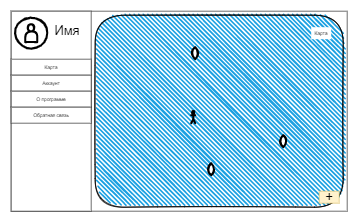
\includegraphics[width=12cm]{main_screen_plan}
	\centering
	\caption*{Приложение А.1. Главный экран клиентского приложения}
\end{figure}

\begin{figure}[!htbp]
	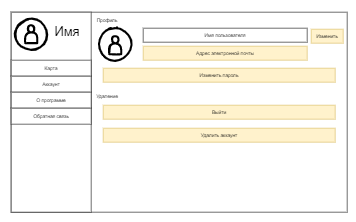
\includegraphics[width=12cm]{account_screen_plan}
	\centering
	\caption*{Приложение А.2. Экран аккаунта пользователя}
\end{figure}

\begin{figure}[!htbp]
	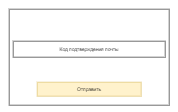
\includegraphics[width=8cm]{code_dialog_plan}
	\centering
	\caption*{Приложение А.3. Диалоговое окно ввода кода}
\end{figure}

\begin{figure}[!htbp]
	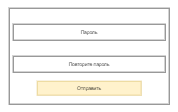
\includegraphics[width=8cm]{password_dialog_plan}
	\centering
	\caption*{Приложение А.4. Диалоговое окно изменения пароля}
\end{figure}

\begin{figure}[!htbp]
	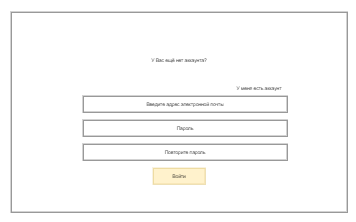
\includegraphics[width=12cm]{auth_screen_plan}
	\centering
	\caption*{Приложение А.5. Экран авторизации}
\end{figure}

\begin{figure}[!htbp]
	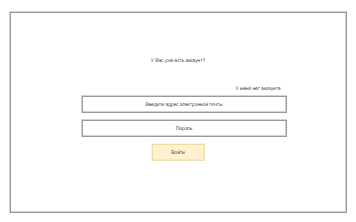
\includegraphics[width=12cm]{login_screen_plan}
	\centering
	\caption*{Приложение А.6. Экран входа в систему}
\end{figure}

\begin{figure}[!htbp]
	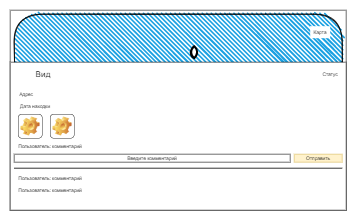
\includegraphics[width=12cm]{view_screen_plan}
	\centering
	\caption*{Приложение А.7. Экран демонстрации отчёта}
\end{figure}

\begin{figure}[!htbp]
	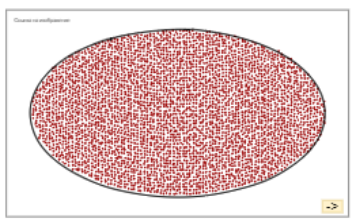
\includegraphics[width=12cm]{full_screen_plan}
	\centering
	\caption*{Приложение А.8. Экран отображения фотографии}
\end{figure}

\begin{figure}[!htbp]
	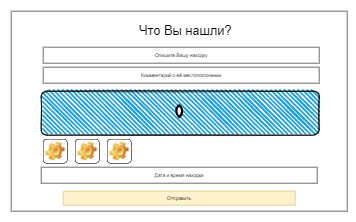
\includegraphics[width=12cm]{report_screen_plan}
	\centering
	\caption*{Приложение А.9. Экран отправки отчёта}
\end{figure}

\begin{figure}[!htbp]
	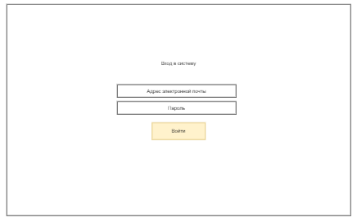
\includegraphics[width=12cm]{login_page_plan}
	\centering
	\caption*{Приложение А.10. Страница входа в систему}
\end{figure}

\begin{figure}[!htbp]
	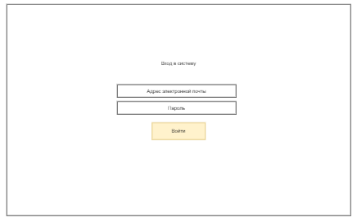
\includegraphics[width=12cm]{login_page_plan}
	\centering
	\caption*{Приложение А.11. Главная страница сервисного сайта}
\end{figure}

\begin{figure}[!htbp]
	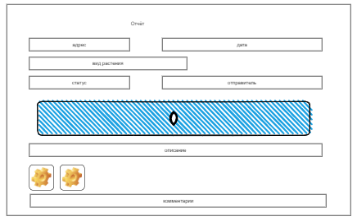
\includegraphics[width=12cm]{report_page_plan}
	\centering
	\caption*{Приложение А.12. Страница редактирования отчёта}
\end{figure}

\begin{figure}[!htbp]
	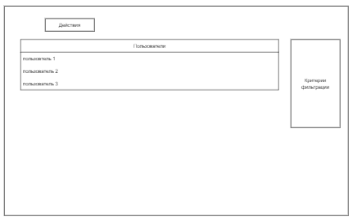
\includegraphics[width=12cm]{users_page_plan}
	\centering
	\caption*{Приложение А.13. Страница отображения пользователей системы}
\end{figure}

\begin{figure}[!htbp]
	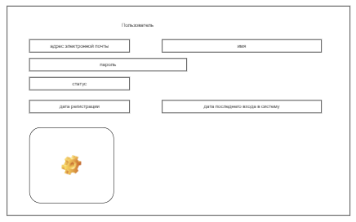
\includegraphics[width=12cm]{user_page_plan}
	\centering
	\caption*{Приложение А.14. Страница редактирования профиля пользователя}
\end{figure}

\begin{figure}[!htbp]
	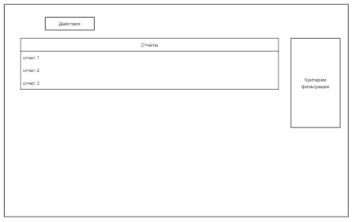
\includegraphics[width=15cm]{reports_page_plan}
	\centering
	\caption*{Приложение А.15. Страница отображения отчётов}
\end{figure}

\cleardoublepage

\addition{interface-real}{Пользовательский интерфейс}

\begin{figure}[!htbp]
	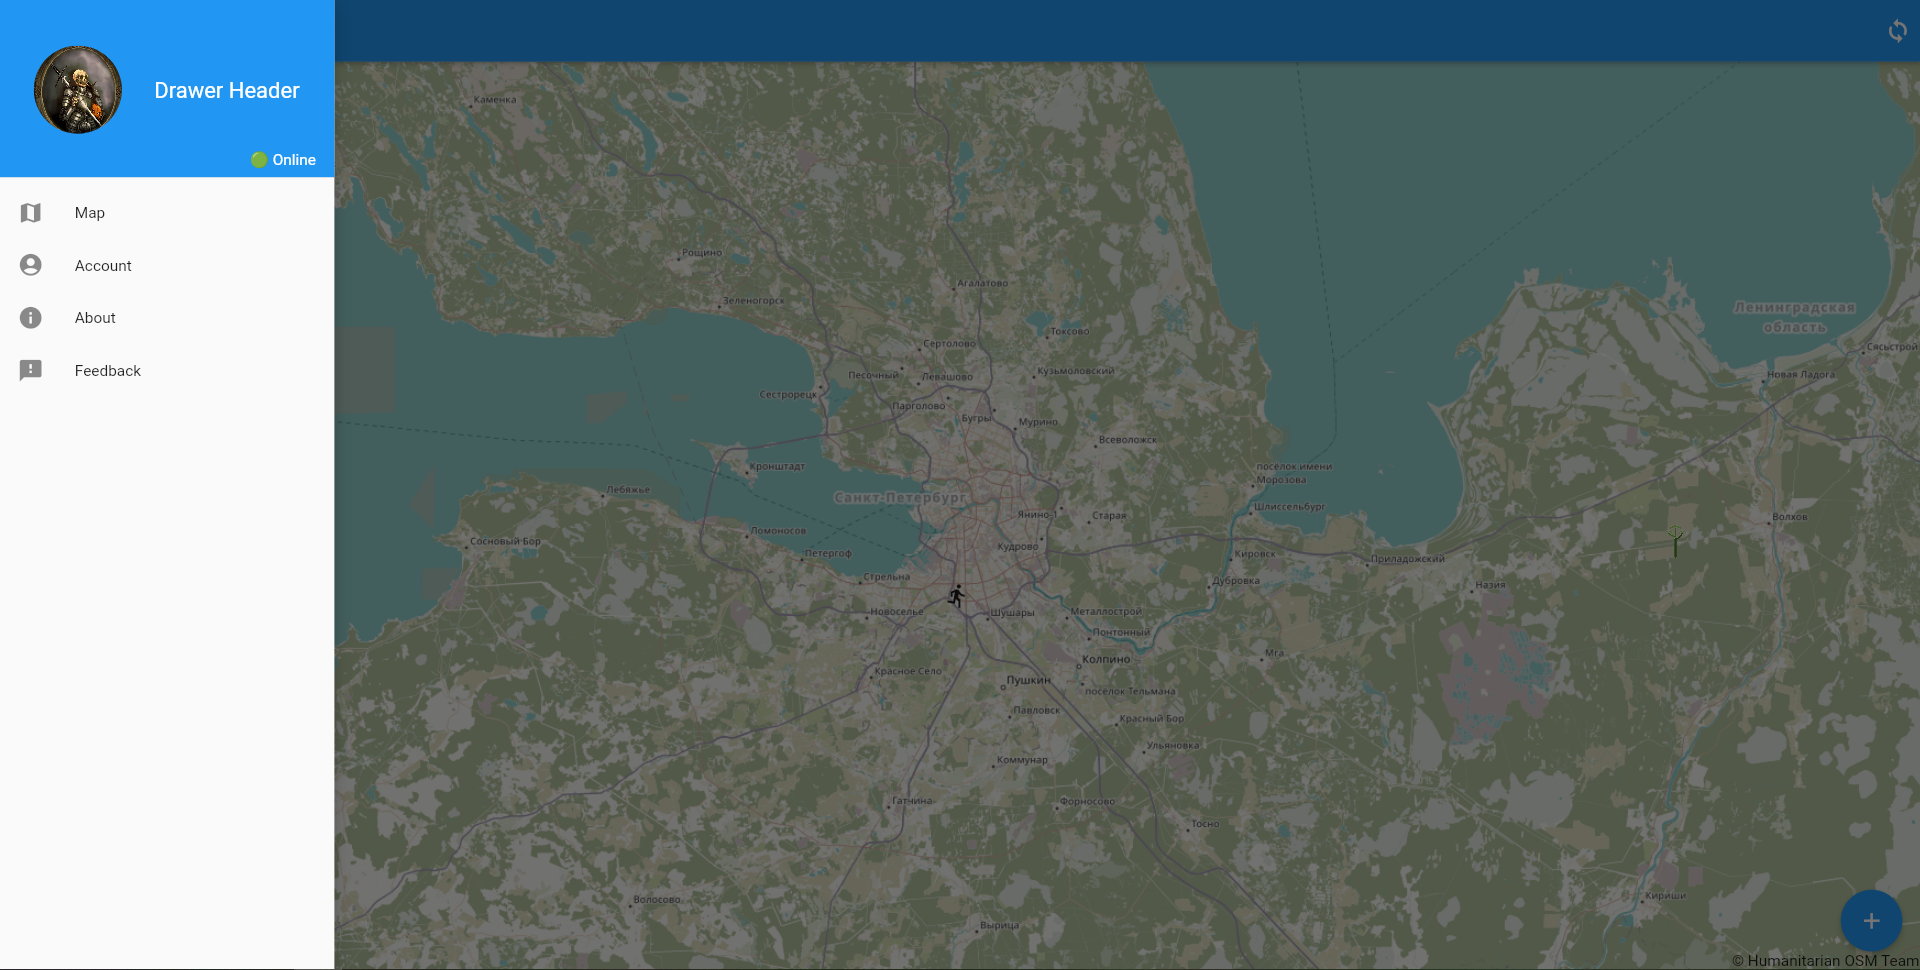
\includegraphics[width=12cm]{main_screen_real}
	\centering
	\caption*{Приложение А.1. Главный экран клиентского приложения}
\end{figure}

\begin{figure}[!htbp]
	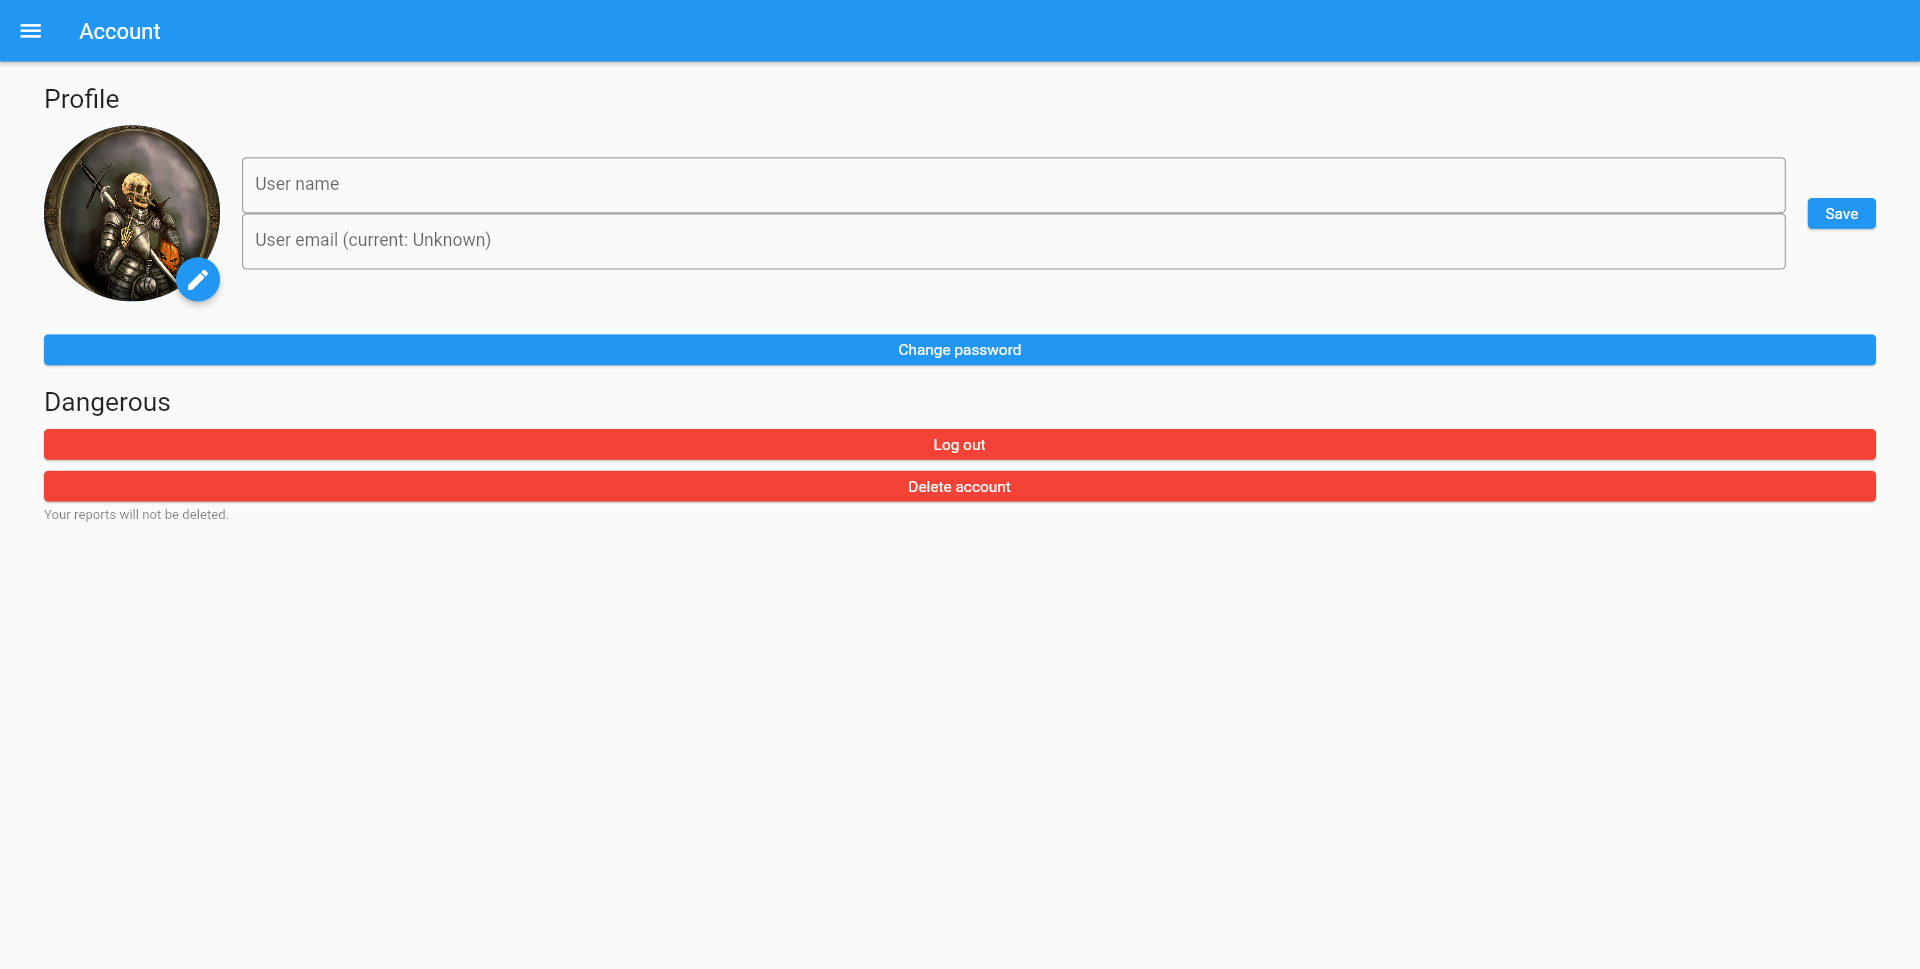
\includegraphics[width=12cm]{account_screen_real}
	\centering
	\caption*{Приложение А.2. Экран аккаунта пользователя}
\end{figure}

\begin{figure}[!htbp]
	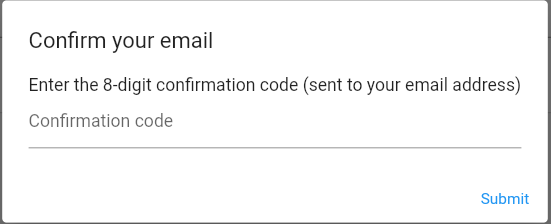
\includegraphics[width=8cm]{code_dialog_real}
	\centering
	\caption*{Приложение А.3. Диалоговое окно ввода кода}
\end{figure}

\begin{figure}[!htbp]
	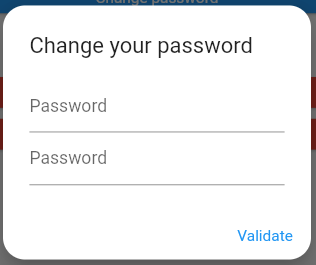
\includegraphics[width=8cm]{password_dialog_real}
	\centering
	\caption*{Приложение А.4. Диалоговое окно изменения пароля}
\end{figure}

\begin{figure}[!htbp]
	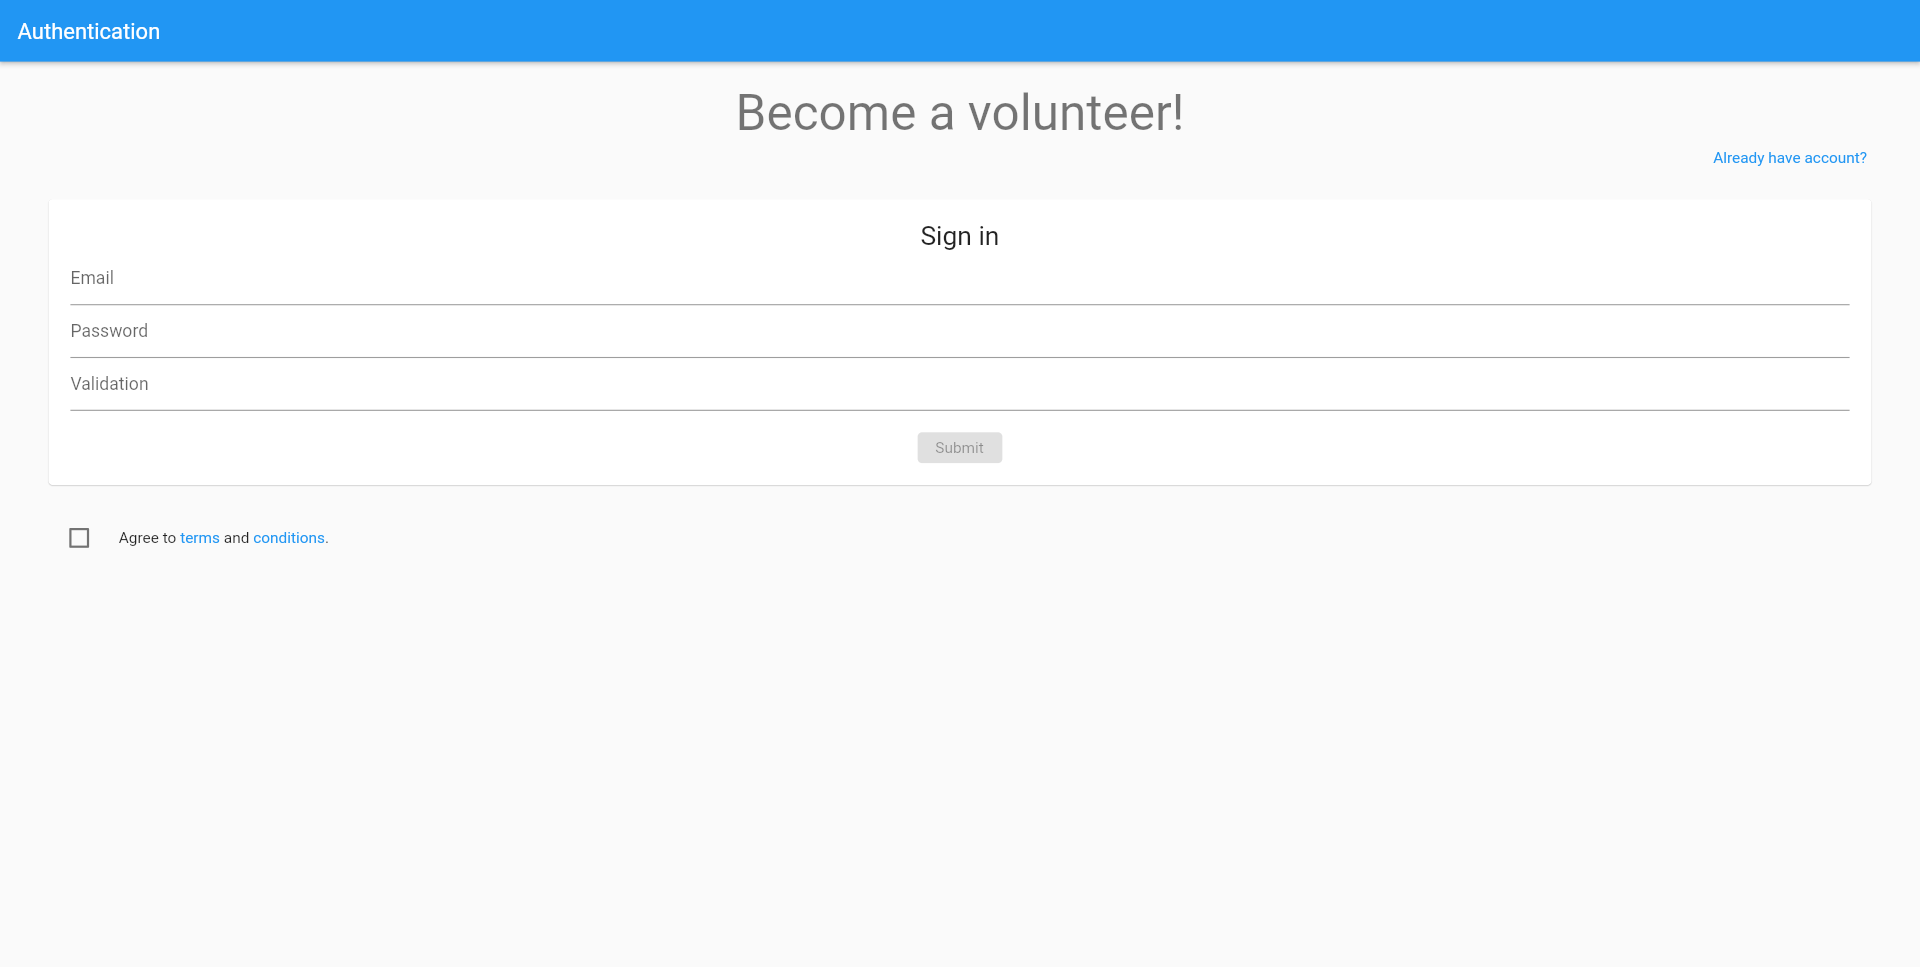
\includegraphics[width=12cm]{auth_screen_real}
	\centering
	\caption*{Приложение А.5. Экран авторизации}
\end{figure}

\begin{figure}[!htbp]
	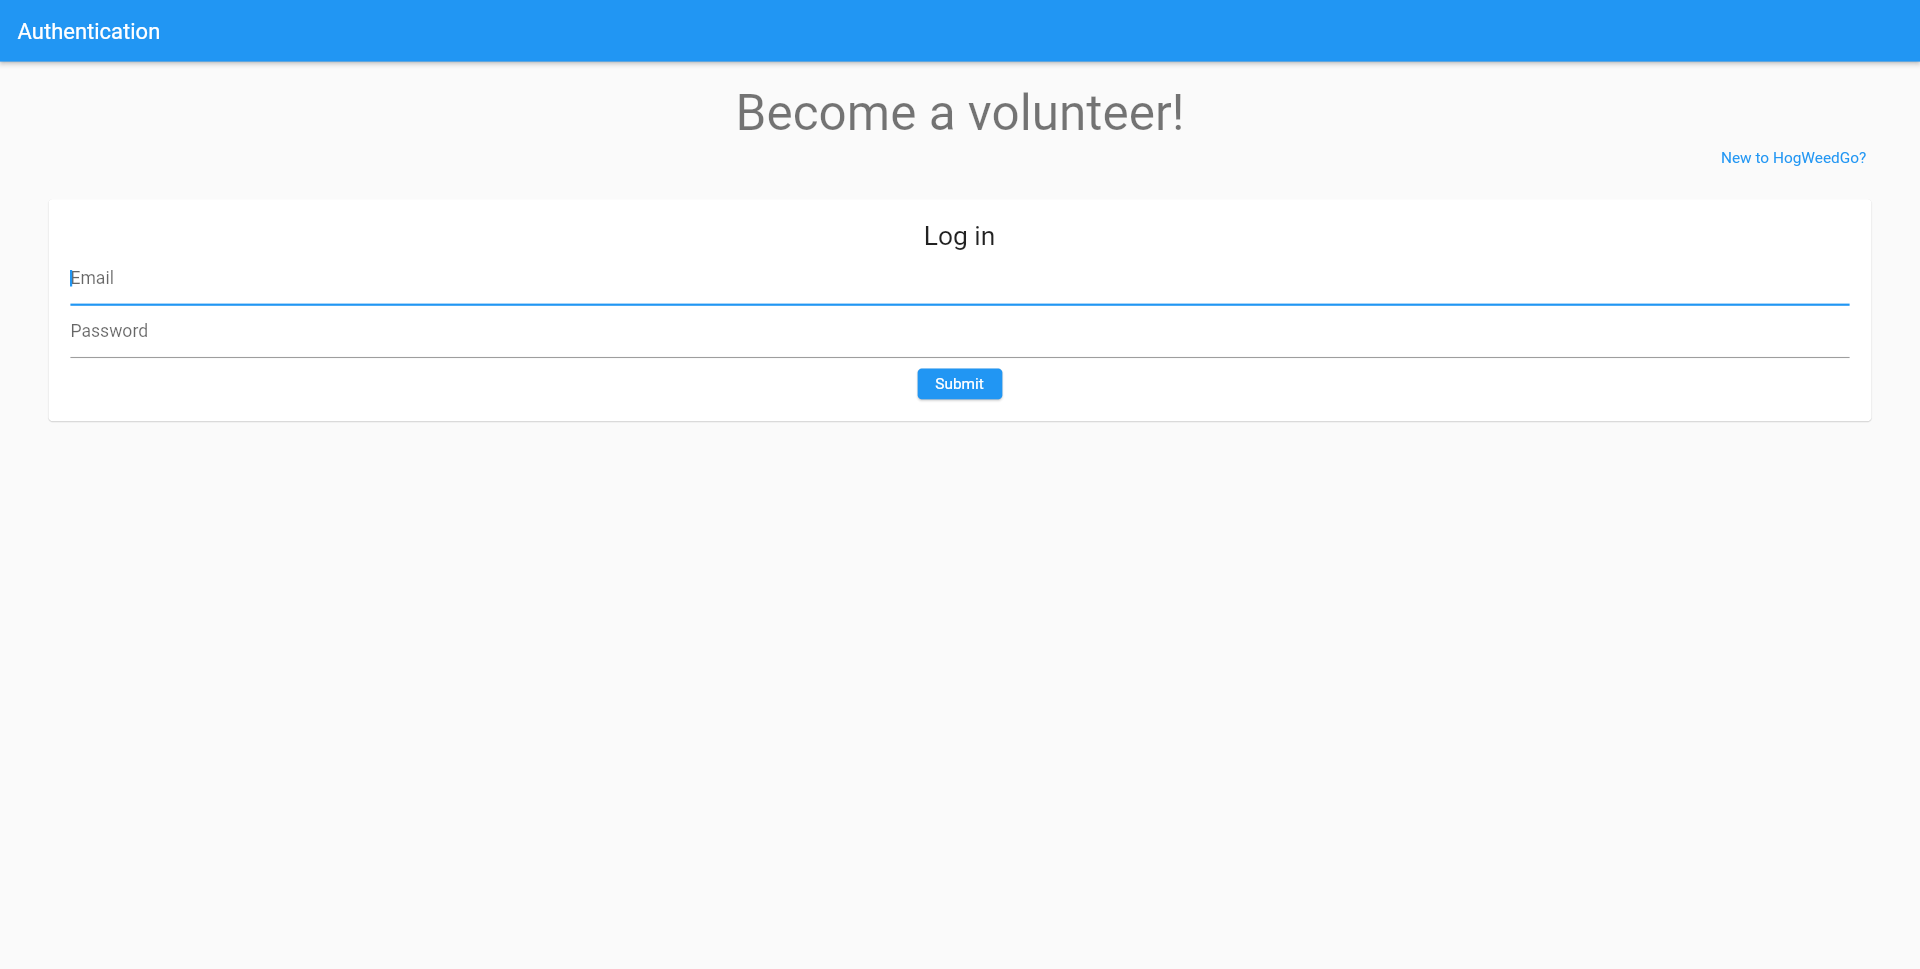
\includegraphics[width=12cm]{login_screen_real}
	\centering
	\caption*{Приложение А.6. Экран входа в систему}
\end{figure}

\begin{figure}[!htbp]
	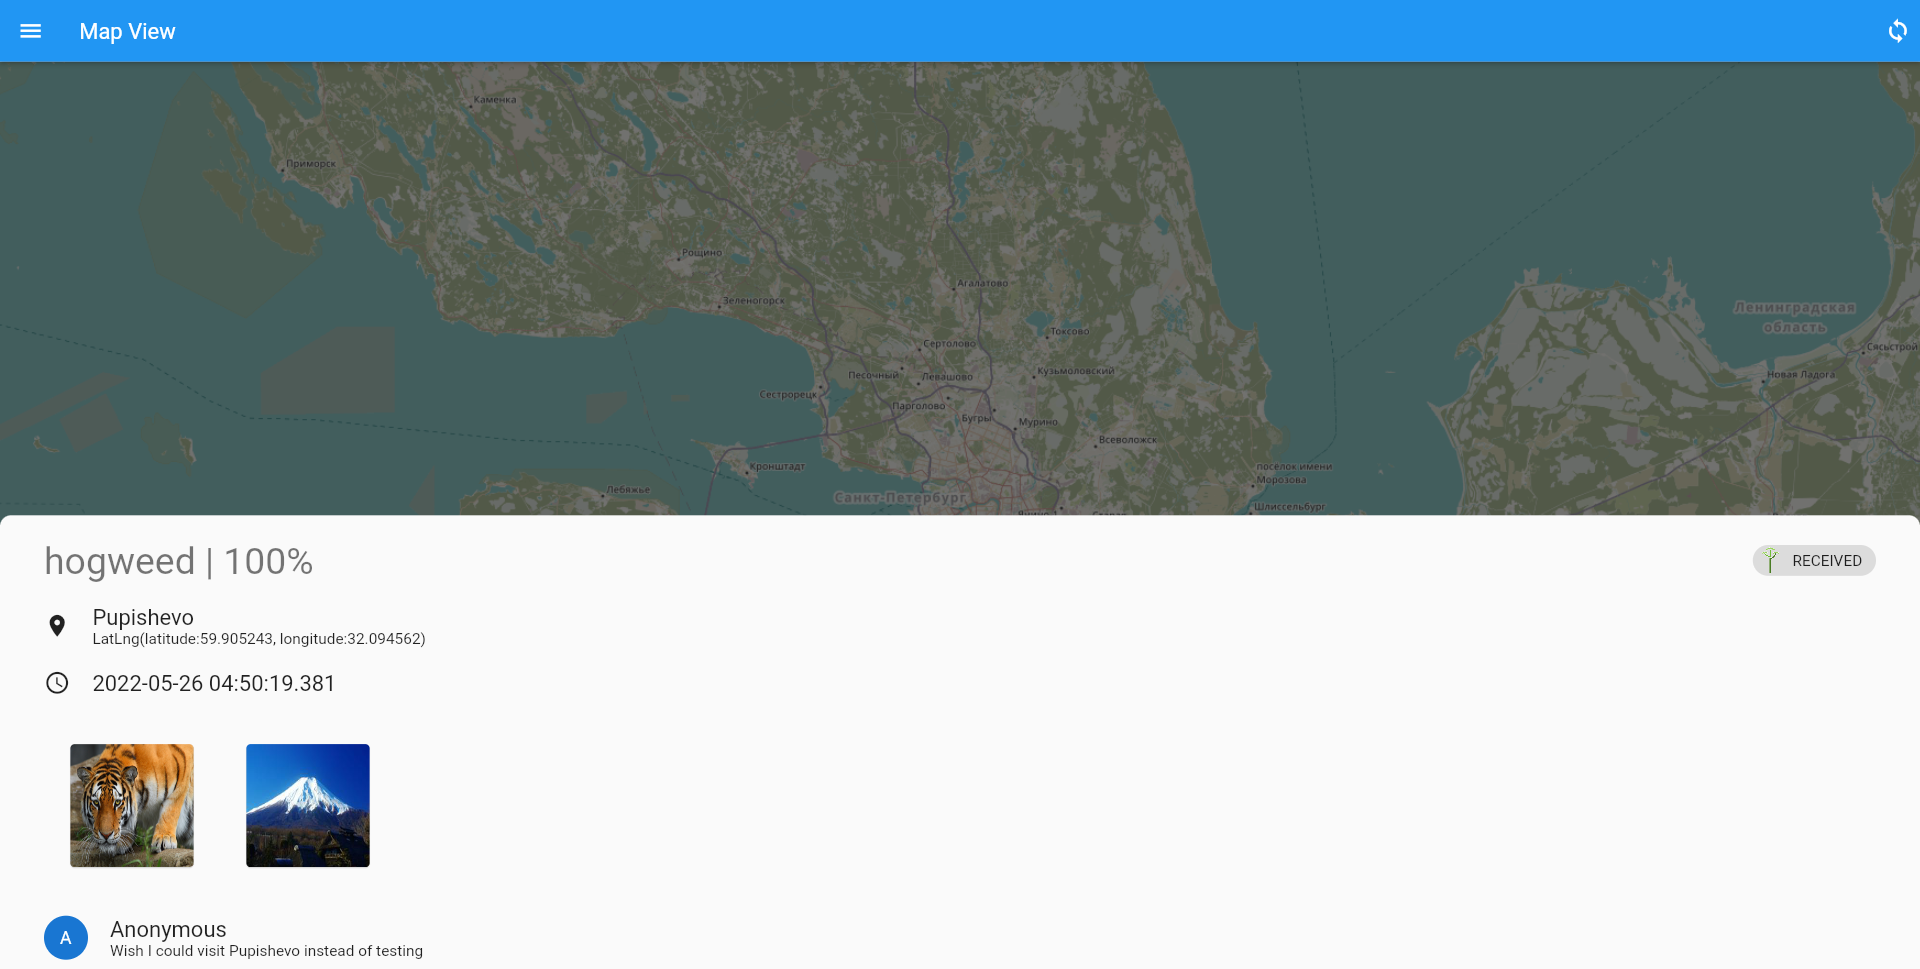
\includegraphics[width=12cm]{view_screen_real}
	\centering
	\caption*{Приложение А.7. Экран демонстрации отчёта}
\end{figure}

\begin{figure}[!htbp]
	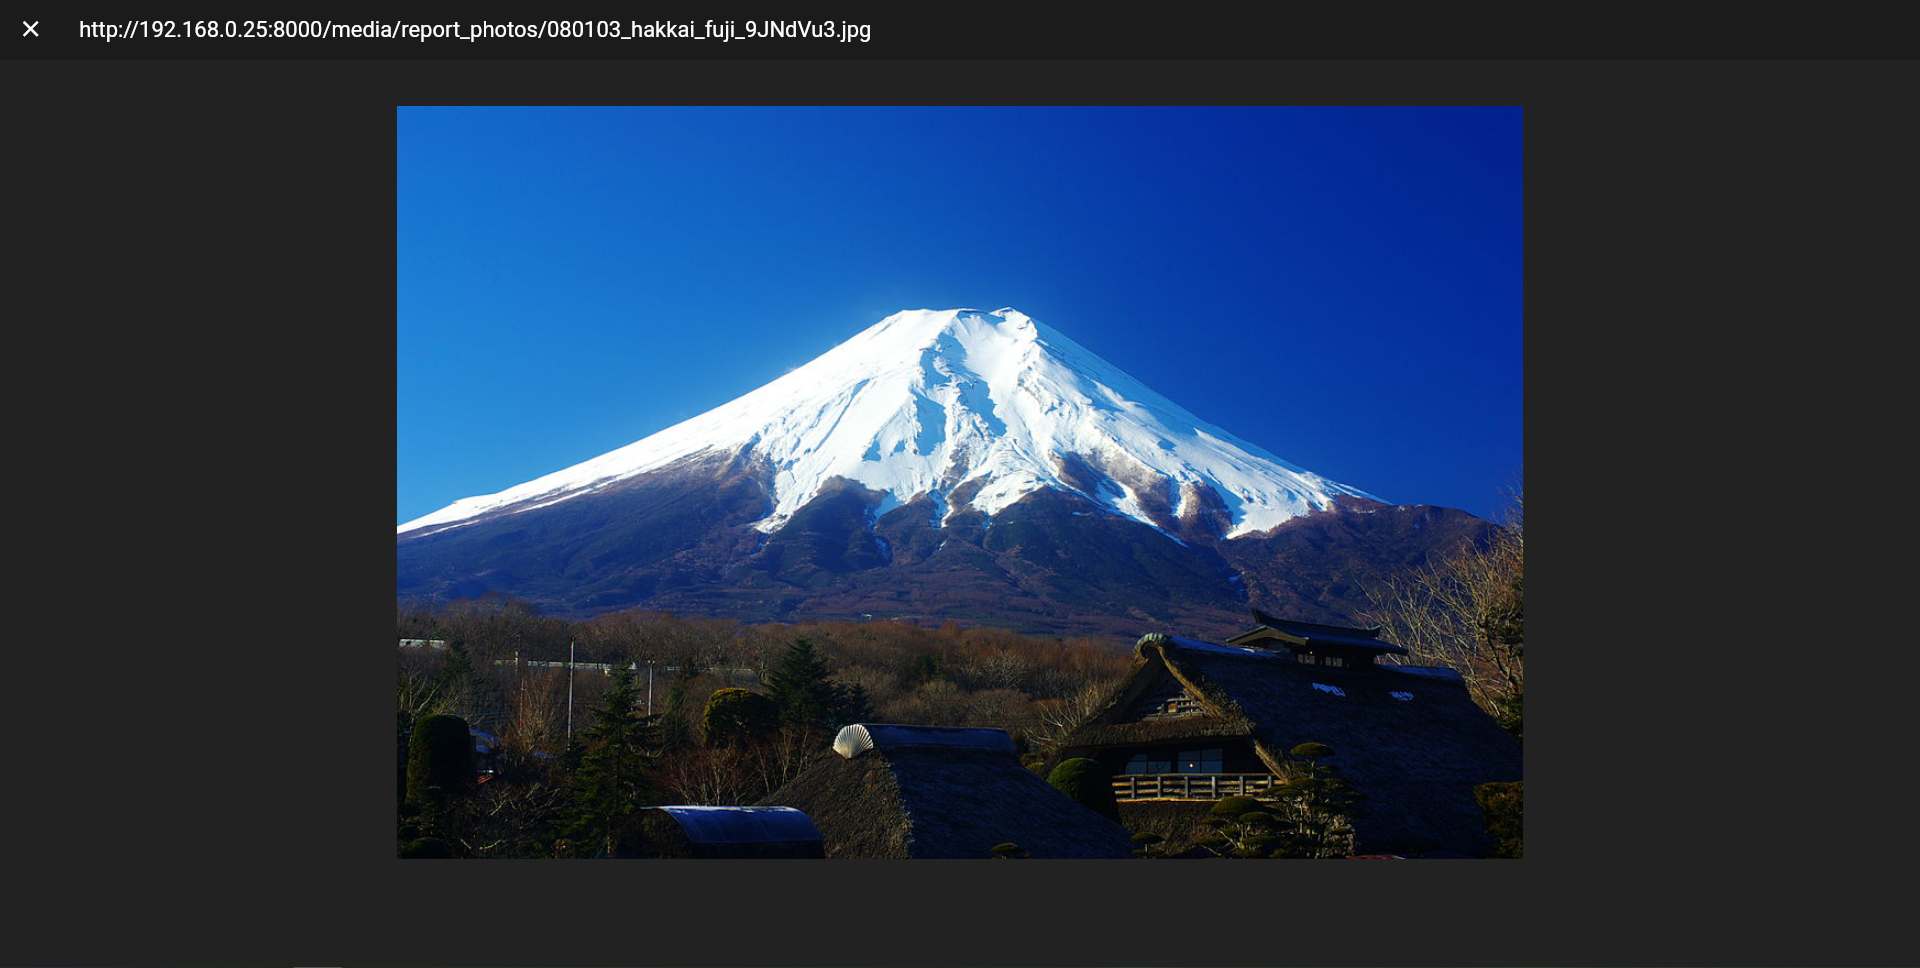
\includegraphics[width=12cm]{full_screen_real}
	\centering
	\caption*{Приложение А.8. Экран отображения фотографии}
\end{figure}

\begin{figure}[!htbp]
	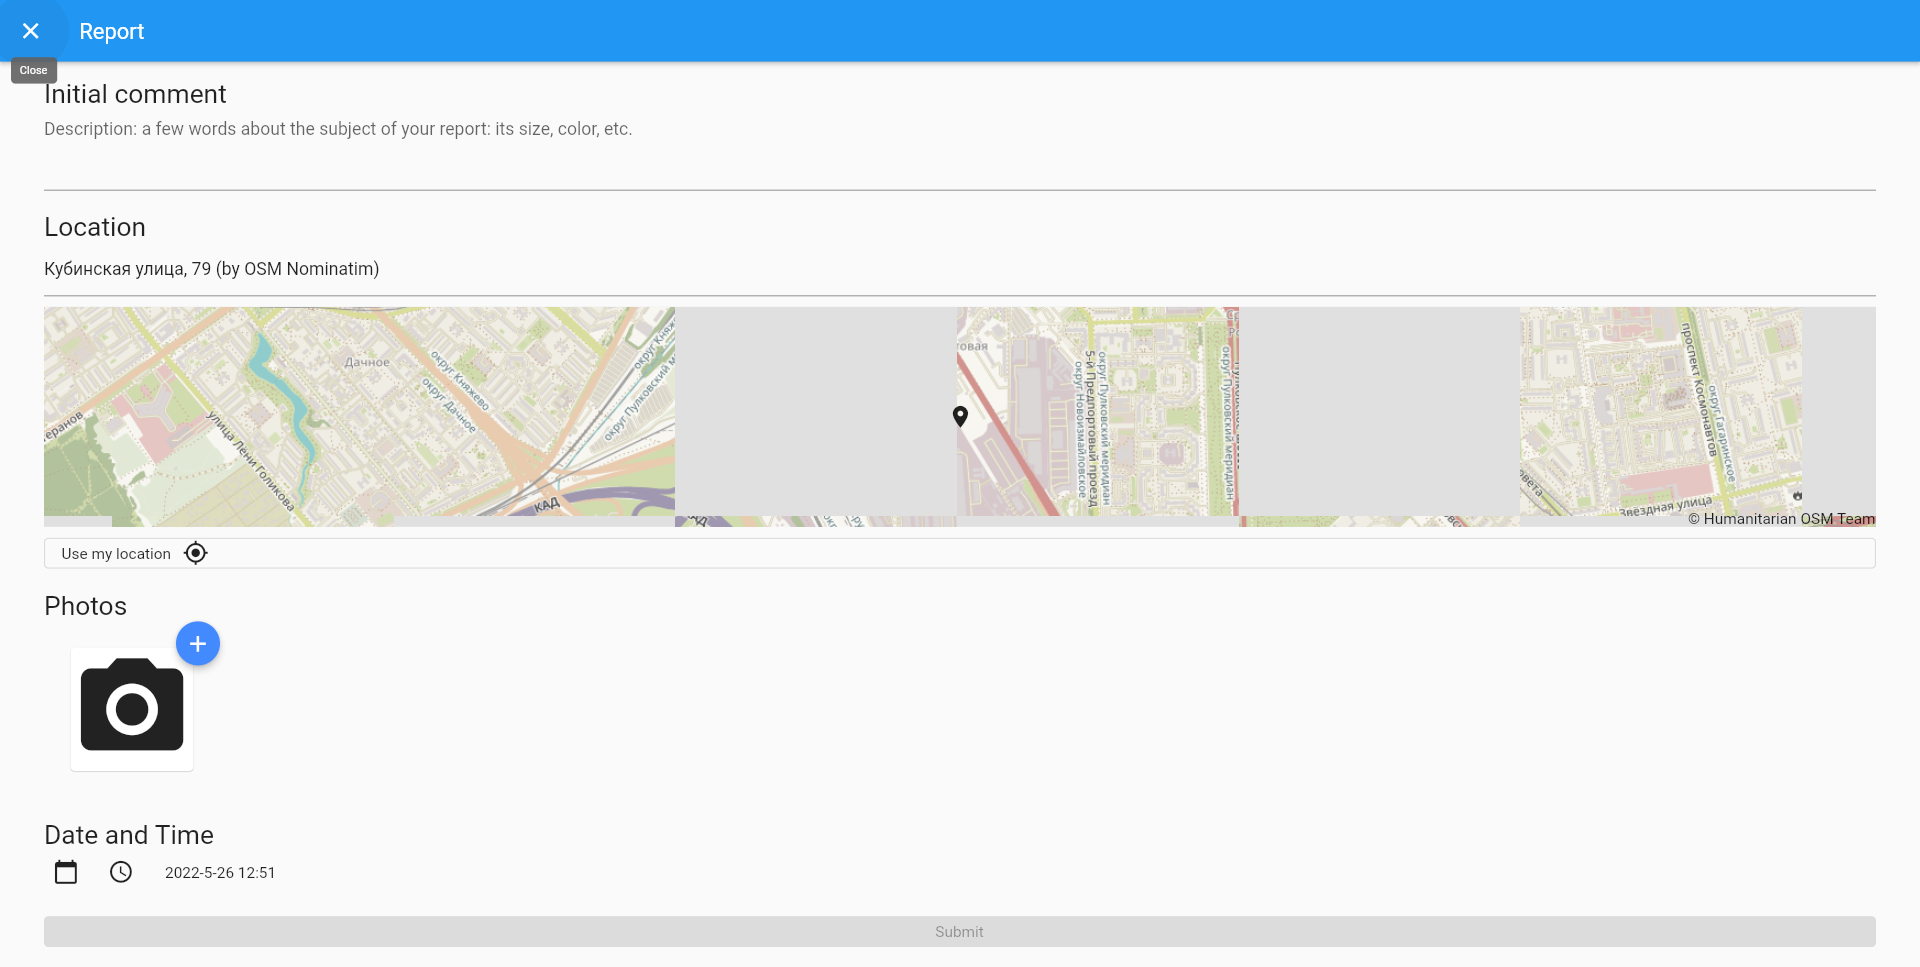
\includegraphics[width=12cm]{report_screen_real}
	\centering
	\caption*{Приложение А.9. Экран отправки отчёта}
\end{figure}

\begin{figure}[!htbp]
	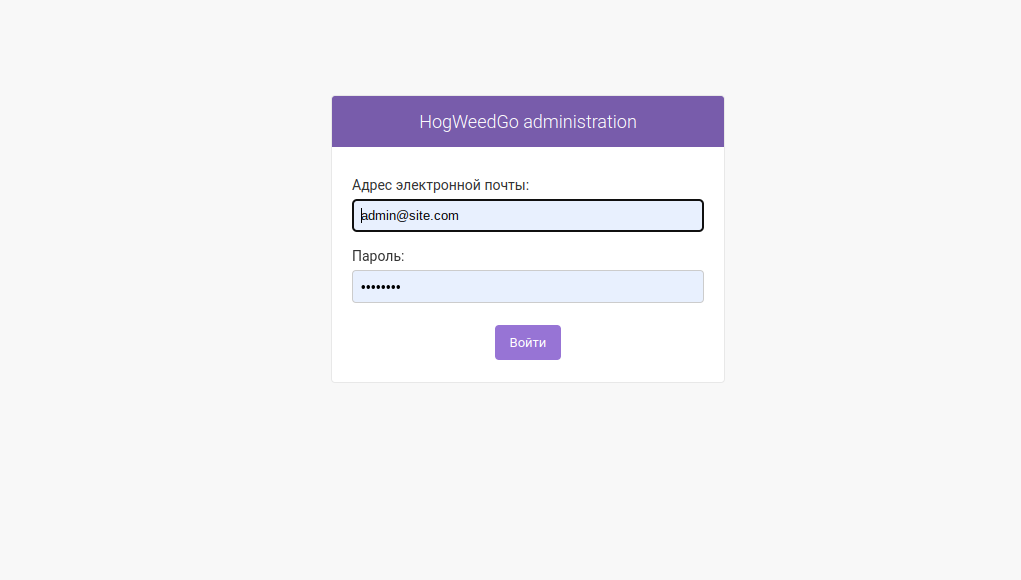
\includegraphics[width=12cm]{login_page_real}
	\centering
	\caption*{Приложение А.10. Страница входа в систему}
\end{figure}

\begin{figure}[!htbp]
	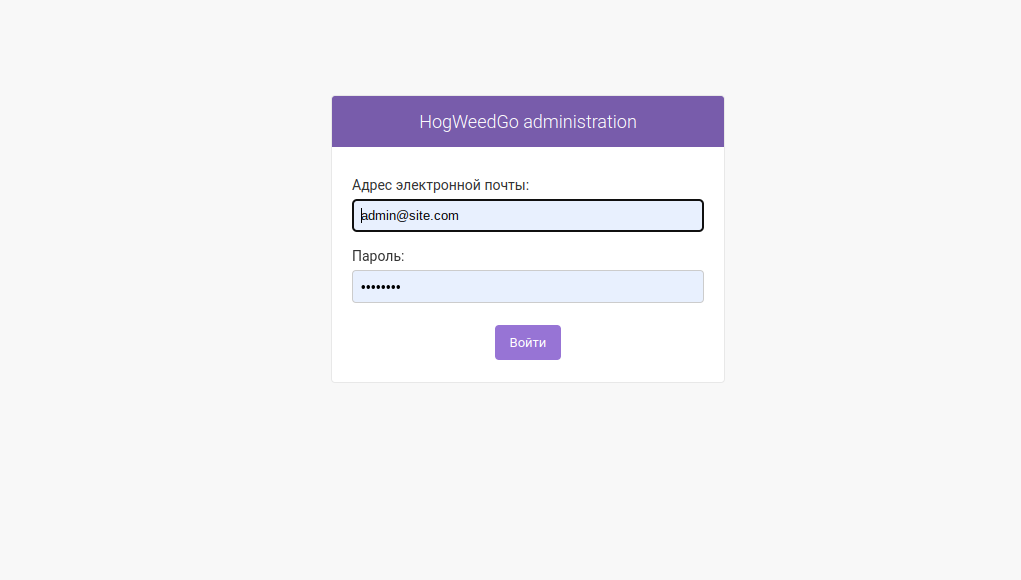
\includegraphics[width=12cm]{login_page_real}
	\centering
	\caption*{Приложение А.11. Главная страница сервисного сайта}
\end{figure}

\begin{figure}[!htbp]
	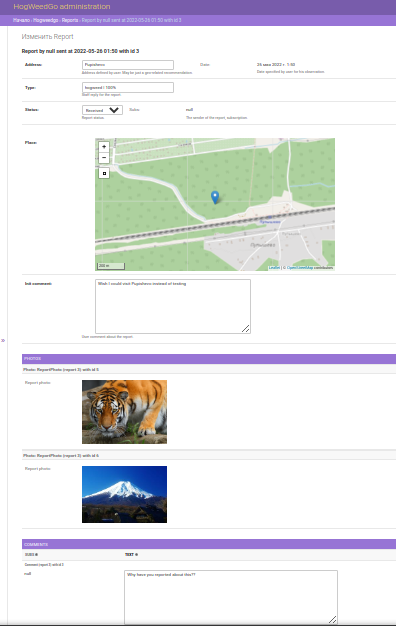
\includegraphics[width=12cm]{report_page_real}
	\centering
	\caption*{Приложение А.12. Страница редактирования отчёта}
\end{figure}

\begin{figure}[!htbp]
	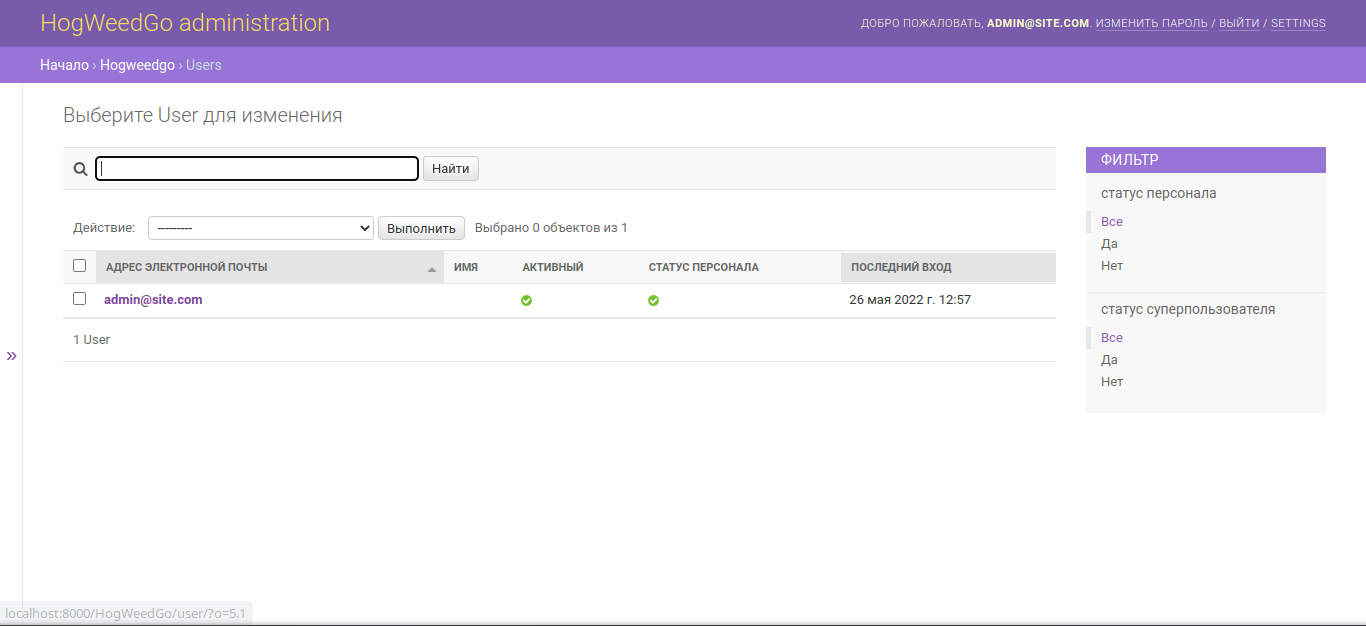
\includegraphics[width=12cm]{users_page_real}
	\centering
	\caption*{Приложение А.13. Страница отображения пользователей системы}
\end{figure}

\begin{figure}[!htbp]
	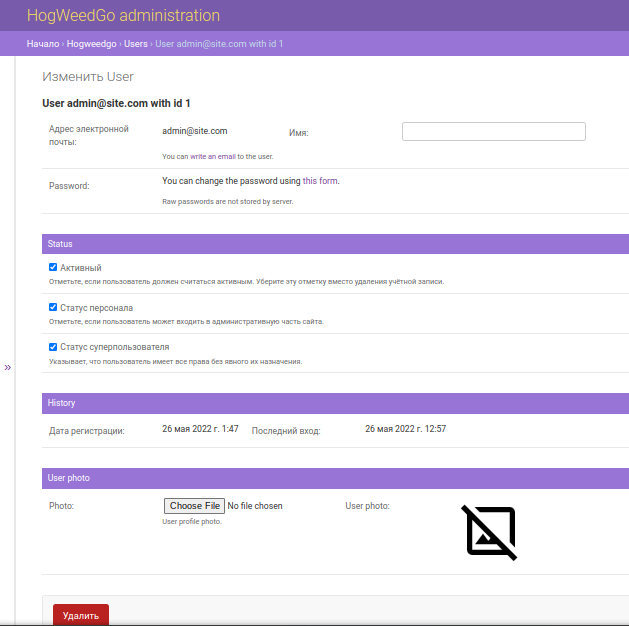
\includegraphics[width=12cm]{user_page_real}
	\centering
	\caption*{Приложение А.14. Страница редактирования профиля пользователя}
\end{figure}

\begin{figure}[!htbp]
	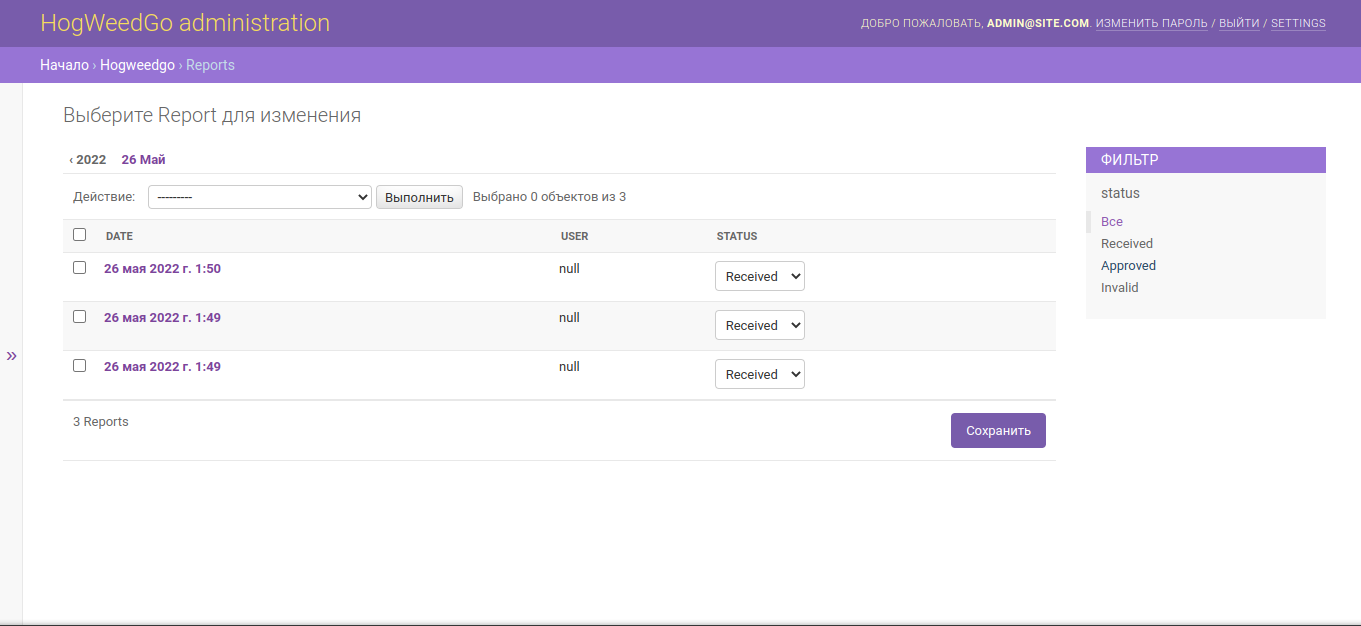
\includegraphics[width=15cm]{reports_page_real}
	\centering
	\caption*{Приложение А.15. Страница отображения отчётов}
\end{figure}

\cleardoublepage

\addition{openapi}{OpenAPI спецификация API системы}

\lstinputlisting[breaklines=true, basicstyle=\small]{../HogWeedGo.openapi.yml}

\end{document}
